\documentclass{article}
\usepackage[a4paper,hmargin=2cm,top=2.25cm,bottom=3cm]{geometry}
\usepackage{graphicx} % Required for inserting images

\usepackage{url}
\bibliographystyle{apalike}
\usepackage{hyperref}
\usepackage[table,xcdraw]{xcolor}
\usepackage{fancyvrb}
\usepackage{minted}
\usepackage{amsmath}
\usepackage{cleveref}
\usepackage{subcaption}
\usepackage{dirtytalk}
\usepackage{parskip}
\usepackage{colortbl}
\usepackage{multirow}
\usepackage{booktabs}
\usepackage{multicol}
\usepackage{makecell}

\usepackage{cleveref}
\usepackage{verbatim}
\usepackage{appendix}
\usepackage{listings}
\usepackage{amsfonts,amsthm}
\usepackage{tikz}
\usetikzlibrary{positioning,shapes,arrows}
\lstset{breaklines=true, basicstyle=\ttfamily}

\usepackage{algorithm}
\usepackage{algpseudocode}

\setlength\parskip{2ex plus 0.2ex minus 0.4ex}
\setlength\parindent{0em}

\DeclareCaptionSubType[alph]{listing}



% \title{PAR Exercise 1. Mining Robot Task.}
% \author{Andreu Garcies Ramon\\Maria Guasch Torres}
% \date{October 2025}

\title{
    \textbf{A3: Epidemic Spreading on Complex Networks}\\
    \large Complex Networks\\
    \small Universitat Rovira i Virgili (URV)\\
    \small Master in Artificial Intelligence (MAI)
}
\author{
    Andreu Garcies Ramon\\
    \texttt{andreu.garcies@estudiantat.upc.edu}
    \and
    Maria Guasch Torres\\
    \texttt{maria.guasch.t@estudiantat.upc.edu}
}
\date{April 2026}

% \bibliographystyle{apa}

\begin{document}


\maketitle

\section{Introduction}

\section{The SIS model}

The Susceptible-Infected-Susceptible (SIS) model is one of the simplest compartmental models for epidemic spreading. Each node in the network occupies one of two states at any given time:

\begin{itemize}
    \item \textbf{Susceptible (S):} the node is healthy but can be infected.
    \item \textbf{Infected (I):} the node carries the disease and can transmit it to neighbors.
\end{itemize}

The dynamics are governed by two parameters:
\begin{enumerate}
    \item $\beta \in [0,1]$ is the transmission probability: at each discrete time step, an infected node transmits the disease to each susceptible neighbour independently with probability $\beta$.
    \item $\mu \in [0,1]$ is the recovery probability: at each time step, an infected node recovers (returns to the susceptible state) with probability $\mu$. Because recovered nodes are susceptible again, the model admits a stationary endemic state in which a non-zero fraction of the population remains infected indefinitely.
\end{enumerate} 

The key macroscopic observable is the stationary infection density (the parameter that we will estimate in the experiments):
\begin{equation}
    \rho = \frac{1}{N}\sum_{i=1}^{N} \rho_i,
\end{equation}
where $\rho_i$ is the long-run probability that node $i$ is infected. An important characteristic of the SIS model is the existence of an epidemic threshold $\beta_c$. For $\beta < \beta_c$ the disease dies out ($\rho \to 0$), while for $\beta > \beta_c$ it persists at a positive endemic level.

\subsection{Monte Carlo simulations}

Monte Carlo (MC) simulations implement the SIS dynamics stochastically and average the resulting infection density over many independent realizations. The simulation is run for $T_{\max}$ time steps per realisation. The first $T_{\text{trans}}$ steps are discarded as a transient, and $\rho$ is estimated by averaging over the remaining $T_{\max} - T_{\text{trans}}$ steps. The procedure is repeated over $N_{\text{rep}}$ independent realizations, each starting from a fresh random infection of a fraction $R_0$ of nodes, and the final estimate is the mean over all realizations.

Algorithm~\ref{alg:sis_naive} shows the straightforward implementation. At each time step, the algorithm iterates over every susceptible node and checks, for each of its neighbors, whether that neighbour is infected and whether transmission occurs. The inner loop therefore touches every edge incident to a susceptible node, yielding a per-step cost of $O(N + E)$. With $N_{\text{rep}} \times T_{\max}$ steps across all realizations the total cost is $O(N_{\text{rep}} \cdot T_{\max} \cdot (N + E))$.

\begin{algorithm}[ht]
\caption{SIS Monte Carlo simulation (naive)}
\label{alg:sis_naive}
\begin{algorithmic}[1]
\Require Graph $G=(V,E)$, infection probability $\beta$, recovery probability $\mu$, repetitions $N_{\text{rep}}$, initial fraction $R_0$, steps $T_{\max}$, transient $T_{\text{trans}}$
\Ensure  Stationary infection density $\rho$

\State $\rho_{\text{avg}} \gets 0$
\For{$\text{rep} = 1$ \textbf{to} $N_{\text{rep}}$}
    \State $\text{infected} \gets \text{random sample of } \lfloor R_0 \cdot N \rfloor \text{ nodes}$
    \State $\text{susceptible} \gets V \setminus \text{infected}$
    \State $\rho_{\text{rep}} \gets 0$
    \For{$t = 1$ \textbf{to} $T_{\max}$}
        \If{$\text{infected} = \emptyset$} \textbf{break} \EndIf
        \State $\text{recoveries} \gets \emptyset$
        \For{$v \in \text{infected}$}
            \If{$\text{random}() < \mu$} \quad $\text{recoveries} \gets \text{recoveries} \cup \{v\}$ \EndIf
        \EndFor
        \State $\text{new\_infected} \gets \emptyset$
        \For{$v \in \text{susceptible}$}
            \For{$u \in \mathcal{N}(v)$}
                \If{$u \in \text{infected}$ \textbf{and} $\text{random}() < \beta$}
                    \State $\text{new\_infected} \gets \text{new\_infected} \cup \{v\}$
                    \State \textbf{break}
                \EndIf
            \EndFor
        \EndFor
        \If{$t > T_{\text{trans}}$}
            \State $\rho_{\text{rep}} \gets \rho_{\text{rep}} + |\text{infected}| / N$
        \EndIf
        \State $\text{infected} \gets (\text{infected} \setminus \text{recoveries}) \cup \text{new\_infected}$
        \State $\text{susceptible} \gets (\text{susceptible} \setminus \text{new\_infected}) \cup \text{recoveries}$
    \EndFor
    \State $\rho_{\text{avg}} \gets \rho_{\text{avg}} + \rho_{\text{rep}} / (T_{\max} - T_{\text{trans}})$
\EndFor
\State \Return $\rho_{\text{avg}} / N_{\text{rep}}$
\end{algorithmic}
\end{algorithm}

The parameters used throughout this work are $N_{\text{rep}} = 100$, $R_0 = 0.2$, $T_{\max} = 1000$, and $T_{\text{trans}} = 900$, giving 100 post-transient steps per realisation.

\subsection{Microscopic Markov Chain Approach (MMCA)}
\textcolor{red}{AIXÒ S'HA DE REVISAR, ESTÀ EXTRET DE LA INFO DEL CHAT. SEGONS EL QUE HI HA IMPLEMENTAT, AQUEST S'AJUSTA MÉS A LES NOSTRES DADES}
The MMCA \cite{gomez2010discrete} provides a deterministic approximation to the SIS dynamics by tracking, for each node $i$, the probability $\rho_i^{(t)}$ of being infected at time $t$. The update equation is obtained by writing the Markov transitions exactly:
\begin{equation}
    \rho_i^{(t+1)} = \rho_i^{(t)}(1-\mu) + \bigl(1 - \rho_i^{(t)}\bigr) \left[1 - \prod_{j \in \mathcal{N}(i)}\!\bigl(1 - \beta\rho_j^{(t)}\bigr)\right].
\end{equation}

The first term on the right accounts for infected nodes that do not recover. The second term accounts for susceptible nodes ($1 - \rho_i^{(t)}$) that are infected by at least one neighbour. The key assumption is that the states of different nodes are statistically independent, which allows the joint probability of escaping infection from all neighbors to be factored as a product. Unlike mean-field approaches that linearise this product, MMCA retains the full product form, making it exact on trees and a good approximation on locally tree-like networks.

Starting from $\rho_i^{(0)} = 0.5$ for all $i$, the iteration is run until
\begin{equation}
    \max_i \bigl|\rho_i^{(t+1)} - \rho_i^{(t)}\bigr| < \varepsilon,
\end{equation}
with $\varepsilon = 10^{-10}$, and the global density $\rho = \tfrac{1}{N}\sum_i \rho_i$ is recorded.

For computational efficiency the product over neighbors is evaluated using the log-sum trick:
\begin{equation}
    \prod_{j \in \mathcal{N}(i)} (1 - \beta\rho_j)
    = \exp\!\left(\sum_j A_{ij}\log(1 - \beta\rho_j)\right)
    = \exp\!\bigl(A \cdot \log(1 - \beta\rho)\bigr)_i,
\end{equation}
reducing the per-iteration cost to a single sparse matrix--vector multiplication.

Linearizing the update equation around $\rho = 0$ shows that the endemic fixed point bifurcates when the spectral radius of $\beta A$ equals $\mu$, yielding the epidemic threshold
\begin{equation}
    \beta_c^{\text{MMCA}} = \frac{\mu}{\lambda_{\max}(A)}.
\end{equation}

\subsection{Quenched Mean Field (QMF)}
\textcolor{red}{AIXÒ S'HA DE REVISAR, ESTÀ EXTRET DE LA INFO DEL CHAT.}
The QMF approach \cite{wang2003epidemic,chakrabarti2008epidemic} also retains the full adjacency matrix but replaces the product infection probability with a linear mean-field approximation. Writing the continuous-time rate equation:
\begin{equation}
    \frac{d\rho_i}{dt} = -\mu\rho_i + \beta(1-\rho_i)\sum_j A_{ij}\rho_j,
\end{equation}
the term $\beta\sum_j A_{ij}\rho_j$ acts as the effective force of infection on node $i$. Setting $d\rho_i/dt = 0$ and defining $\theta_i = \sum_j A_{ij}\rho_j = (A\rho)_i$ yields the self-consistent fixed-point equation:
\begin{equation}
    \rho_i = \frac{\beta\theta_i}{\mu + \beta\theta_i}.
\end{equation}

This is solved by the iteration: initialise $\rho^{(0)} = 0.5$, then alternately compute $\theta = A\rho$ and update $\rho_i \leftarrow \beta\theta_i / (\mu + \beta\theta_i)$ until convergence. Each iteration again requires only a single matrix--vector multiplication.

The epidemic threshold is identical to that of MMCA:
\begin{equation}
    \beta_c^{\text{QMF}} = \frac{\mu}{\lambda_{\max}(A)}.
\end{equation}

Because QMF linearizes the infection probability, it overestimates $\rho$ relative to MMCA for $\beta$ well above threshold. Both methods share the same threshold $\beta_c$, so they agree in the critical region but diverge at higher infection rates.

\section{Networks used}
All experiments are conducted on four networks of $N = 1000$ nodes generated with fixed random seeds for reproducibility.

\textbf{Erdös--Rényi (ER).} In an ER graph $G(N,p)$ each pair of nodes is connected independently with probability $p$. Choosing $p = \langle k \rangle / (N-1)$ targets a given average degree $\langle k \rangle$. The degree distribution follows a Poisson distribution centred on $\langle k \rangle$. The spectral radius satisfies $\lambda_{\max} \approx \langle k \rangle$, and the epidemic threshold scales as $\beta_c \approx \mu / \langle k \rangle$ (Equation 8 in \cite{gomez2010discrete})\textcolor{red}{Aquesta equació més o manco quadra amb els resultats obtinguts. A les comparacions amb els models teòrics, MMCA és més precís que QMF}.

\textbf{Barabási--Albert (BA).} BA graphs are grown by preferential attachment. Each new node attaches $m$ edges to existing nodes with probability proportional to their current degree, producing a power-law degree distribution $P(k) \sim k^{-3}$. $\beta_c$ is lower compared to ER graphs with the same average degree.

Two values of average degree are studied for each model: $\langle k \rangle \approx 4$ and $\langle k \rangle \approx 6$. The detailed statistics of each network are reported in \Cref{tab:networks}.

\begin{table}[ht]
\centering
\begin{tabular}{lrrrrrr}
\toprule
Network & $N$ & $E$ & $\langle k \rangle$ & $\lambda_{\max}$ & $\beta_c$ ($\mu{=}0.2$) & $\beta_c$ ($\mu{=}0.4$) \\
\midrule
ER $\langle k\rangle=4$ & 1000 & 1988 & 3.98 & 5.213 & 0.0384 & 0.0767 \\
ER $\langle k\rangle=6$ & 1000 & 2991 & 5.98 & 7.178 & 0.0279 & 0.0557 \\
BA $\langle k\rangle=4$ & 1000 & 1996 & 3.99 & 10.823 & 0.0185 & 0.0370 \\
BA $\langle k\rangle=6$ & 1000 & 2991 & 5.98 & 14.237 & 0.0140 & 0.0281 \\
\bottomrule
\end{tabular}
\caption{Detailed statistics of the four networks used in the experiments. $\langle k \rangle$ is average degree. $\lambda_{\max}$ is the spectral radius of the adjacency matrix. $\beta_c = \mu / \lambda_{\max}$ is the epidemic threshold.}
\label{tab:networks}
\end{table}

Two key observations can be derived from \Cref{tab:networks}. First, for the same $\langle k \rangle$, BA networks have a much larger $\langle k^2 \rangle$ and $\lambda_{\max}$ than ER networks, reflecting the presence of high-degree hubs. This translates directly into a lower $\beta_c$: BA networks are considerably more vulnerable to epidemic spreading than their ER counterparts. Second, increasing $\langle k \rangle$ from 4 to 6 increases $\lambda_{\max}$ in both models, again lowering the threshold.

\section{Results and Discussion}

\section{Code Efficiency}

The naive Monte Carlo implementation (Algorithm~\ref{alg:sis_naive}) has two main bottlenecks. First, infected and susceptible nodes are stored as Python lists, making membership queries $O(N)$. Second, the inner loop iterates over all susceptible nodes at every time step, even though most of them have no infected neighbour and therefore zero probability of becoming infected.

Algorithm~\ref{alg:sis_opt} shows the optimized implementation that addresses both issues. The optimized algorithm was first written in Python and then translated to C++ without any algorithmic changes~\footnote{Given that this was not the main scope of the project, the translation to C++ was carried out with the use of LLMs.}.

\begin{algorithm}[ht]
\caption{SIS Monte Carlo simulation (optimized)}
\label{alg:sis_opt}
\begin{algorithmic}[1]
\Require Graph $G=(V,E)$, parameters $\beta$, $\mu$, $N_{\text{rep}}$,
         $R_0$, $T_{\max}$, $T_{\text{trans}}$
\Ensure  Stationary infection density $\rho$

\State Pre-compute $\mathcal{N}(v)$ as a \textbf{set} for all $v \in V$ \Comment{done once before the rep loop}
\State $\rho_{\text{avg}} \gets 0$
\For{$\text{rep} = 1$ \textbf{to} $N_{\text{rep}}$}
    \State $\text{infected} \gets $ random sample of $\lfloor R_0 \cdot N \rfloor$ nodes, stored as a \textbf{hash-set}
    \State $\rho_{\text{rep}} \gets 0$
    \For{$t = 1$ \textbf{to} $T_{\max}$}
        \If{$\text{infected} = \emptyset$} \textbf{break} \EndIf
        \State $\text{recoveries} \gets \{v \in \text{infected} : \text{random}() < \mu\}$
        \State $\text{candidates} \gets \bigl(\bigcup_{v \in \text{infected}} \mathcal{N}(v)\bigr) \setminus \text{infected}$
        \Comment{only susceptible neighbors of infected nodes}
        \State $\text{new\_infected} \gets \emptyset$
        \For{$v \in \text{candidates}$}
            \State $m \gets |\mathcal{N}(v) \cap \text{infected}|$ \Comment{number of infected neighbors}
            \If{$\text{random}() < 1 - (1-\beta)^m$}
                \State $\text{new\_infected} \gets \text{new\_infected} \cup \{v\}$
            \EndIf
        \EndFor
        \If{$t \geq T_{\text{trans}}$}
            \State $\rho_{\text{rep}} \gets \rho_{\text{rep}} + |\text{infected}| / N$
        \EndIf
        \State $\text{infected} \gets (\text{infected} \setminus \text{recoveries}) \cup \text{new\_infected}$
    \EndFor
    \State $\rho_{\text{avg}} \gets \rho_{\text{avg}} + \rho_{\text{rep}} / (T_{\max} - T_{\text{trans}})$
\EndFor
\State \Return $\rho_{\text{avg}} / N_{\text{rep}}$
\end{algorithmic}
\end{algorithm}

The optimized version introduces four key changes with respect to the naive one:

\begin{enumerate}
    \item \textbf{Hash-set storage.} The infected set is maintained as a hash-set (Python \texttt{set} / C++ \texttt{unordered\_set}), reducing membership checks from $O(N)$ to $O(1)$.
    \item \textbf{Candidate filtering.} Instead of iterating over all susceptible nodes, only the union of the neighbourhoods of currently infected nodes is considered (line 9). When the epidemic is sparse, this set is much smaller than $N$, providing a large practical speedup.
    \item \textbf{Compound infection probability.} Rather than drawing a separate Bernoulli trial for each infected neighbour, the probability of being infected by at least one of $m$ infected neighbors is computed in closed form as $1-(1-\beta)^m$ (line 12), reducing the number of random number draws.
    \item \textbf{List comprehensions (Python only).} The recoveries and candidate sets are built with Python set/list comprehensions instead of explicit \texttt{for} loops. Comprehensions execute in CPython's internal C loop, which is faster than interpreted Python loops.
\end{enumerate}

\subsection{Timing comparison}


\Cref{tab:timing} reports the total wall-clock time to run all 248 simulation points (4 networks $\times$ 2 values of $\mu$ $\times$ 31 values of $\beta$) with $N_{\text{rep}} = 100$ on the same hardware~\footnote{All simulations were run on a Linux machine, running Ubuntu with an AMD Ryzen 9 7900X 12-core processor}. Three implementations are compared: the naive Python baseline, the optimized Python version applying the three changes described above, and the C++ port of that same optimized algorithm (identical logic, no further algorithmic changes).

\begin{table}[ht]
\centering
\begin{tabular}{lrrr}
    \toprule
    Implementation & Total time & Speedup vs.\ naive & Speedup vs.\ efficient Py \\
    \midrule
    Naive Python      & $\approx\!53544$ s ($\sim$14.9 h) & $1\times$    & ---         \\
    Efficient Python  & $\approx\!4606$ s ($\sim$1.3 h)   & $11.6\times$ & $1\times$   \\
    Efficient C++     & $\approx\!1162$ s ($\sim$19 min)  & $46.1\times$ & $\sim\!4\times$ \\
    \bottomrule
\end{tabular}
\caption{Total wall-clock time for the full simulation campaign (248 points, $N_{\text{rep}}=100$ each). Speedup is relative to the naive Python baseline.}
\label{tab:timing}
\end{table}

The optimized Python implementation is roughly $11.6\times$ faster than the naive version. The C++ implementation applies the same algorithmic optimisations as the efficient Python version, but takes advantage from compiled execution, native data structures, and the absence of interpreter overhead. This yields an additional $\sim\!4\times$ speedup over efficient Python, bringing the total reduction to $\sim\!46\times$ relative to the naive baseline. The C++ run completes all the experiments in under 20 minutes, compared to nearly 15 hours for the naive implementation.

\subsection{Implementation correctness}

Despite the algorithmic differences described above, the three implementations are equivalent. The slight discrepancies visible in \Cref{fig:impl_comparison} are purely due to Monte Carlo sampling variance. Each implementation consumes random numbers at a different rate per time step (the naive version draws up to one number per infected neighbour per susceptible node and the optimized version draws exactly one per candidate), so despite sharing the same initial seed the two random streams diverge immediately, producing different stochastic trajectories. The discrepancy is most visible at large $\beta$, where the endemic state fluctuates more across realizations, amplifying the error.

\begin{figure}[ht]
    \centering
    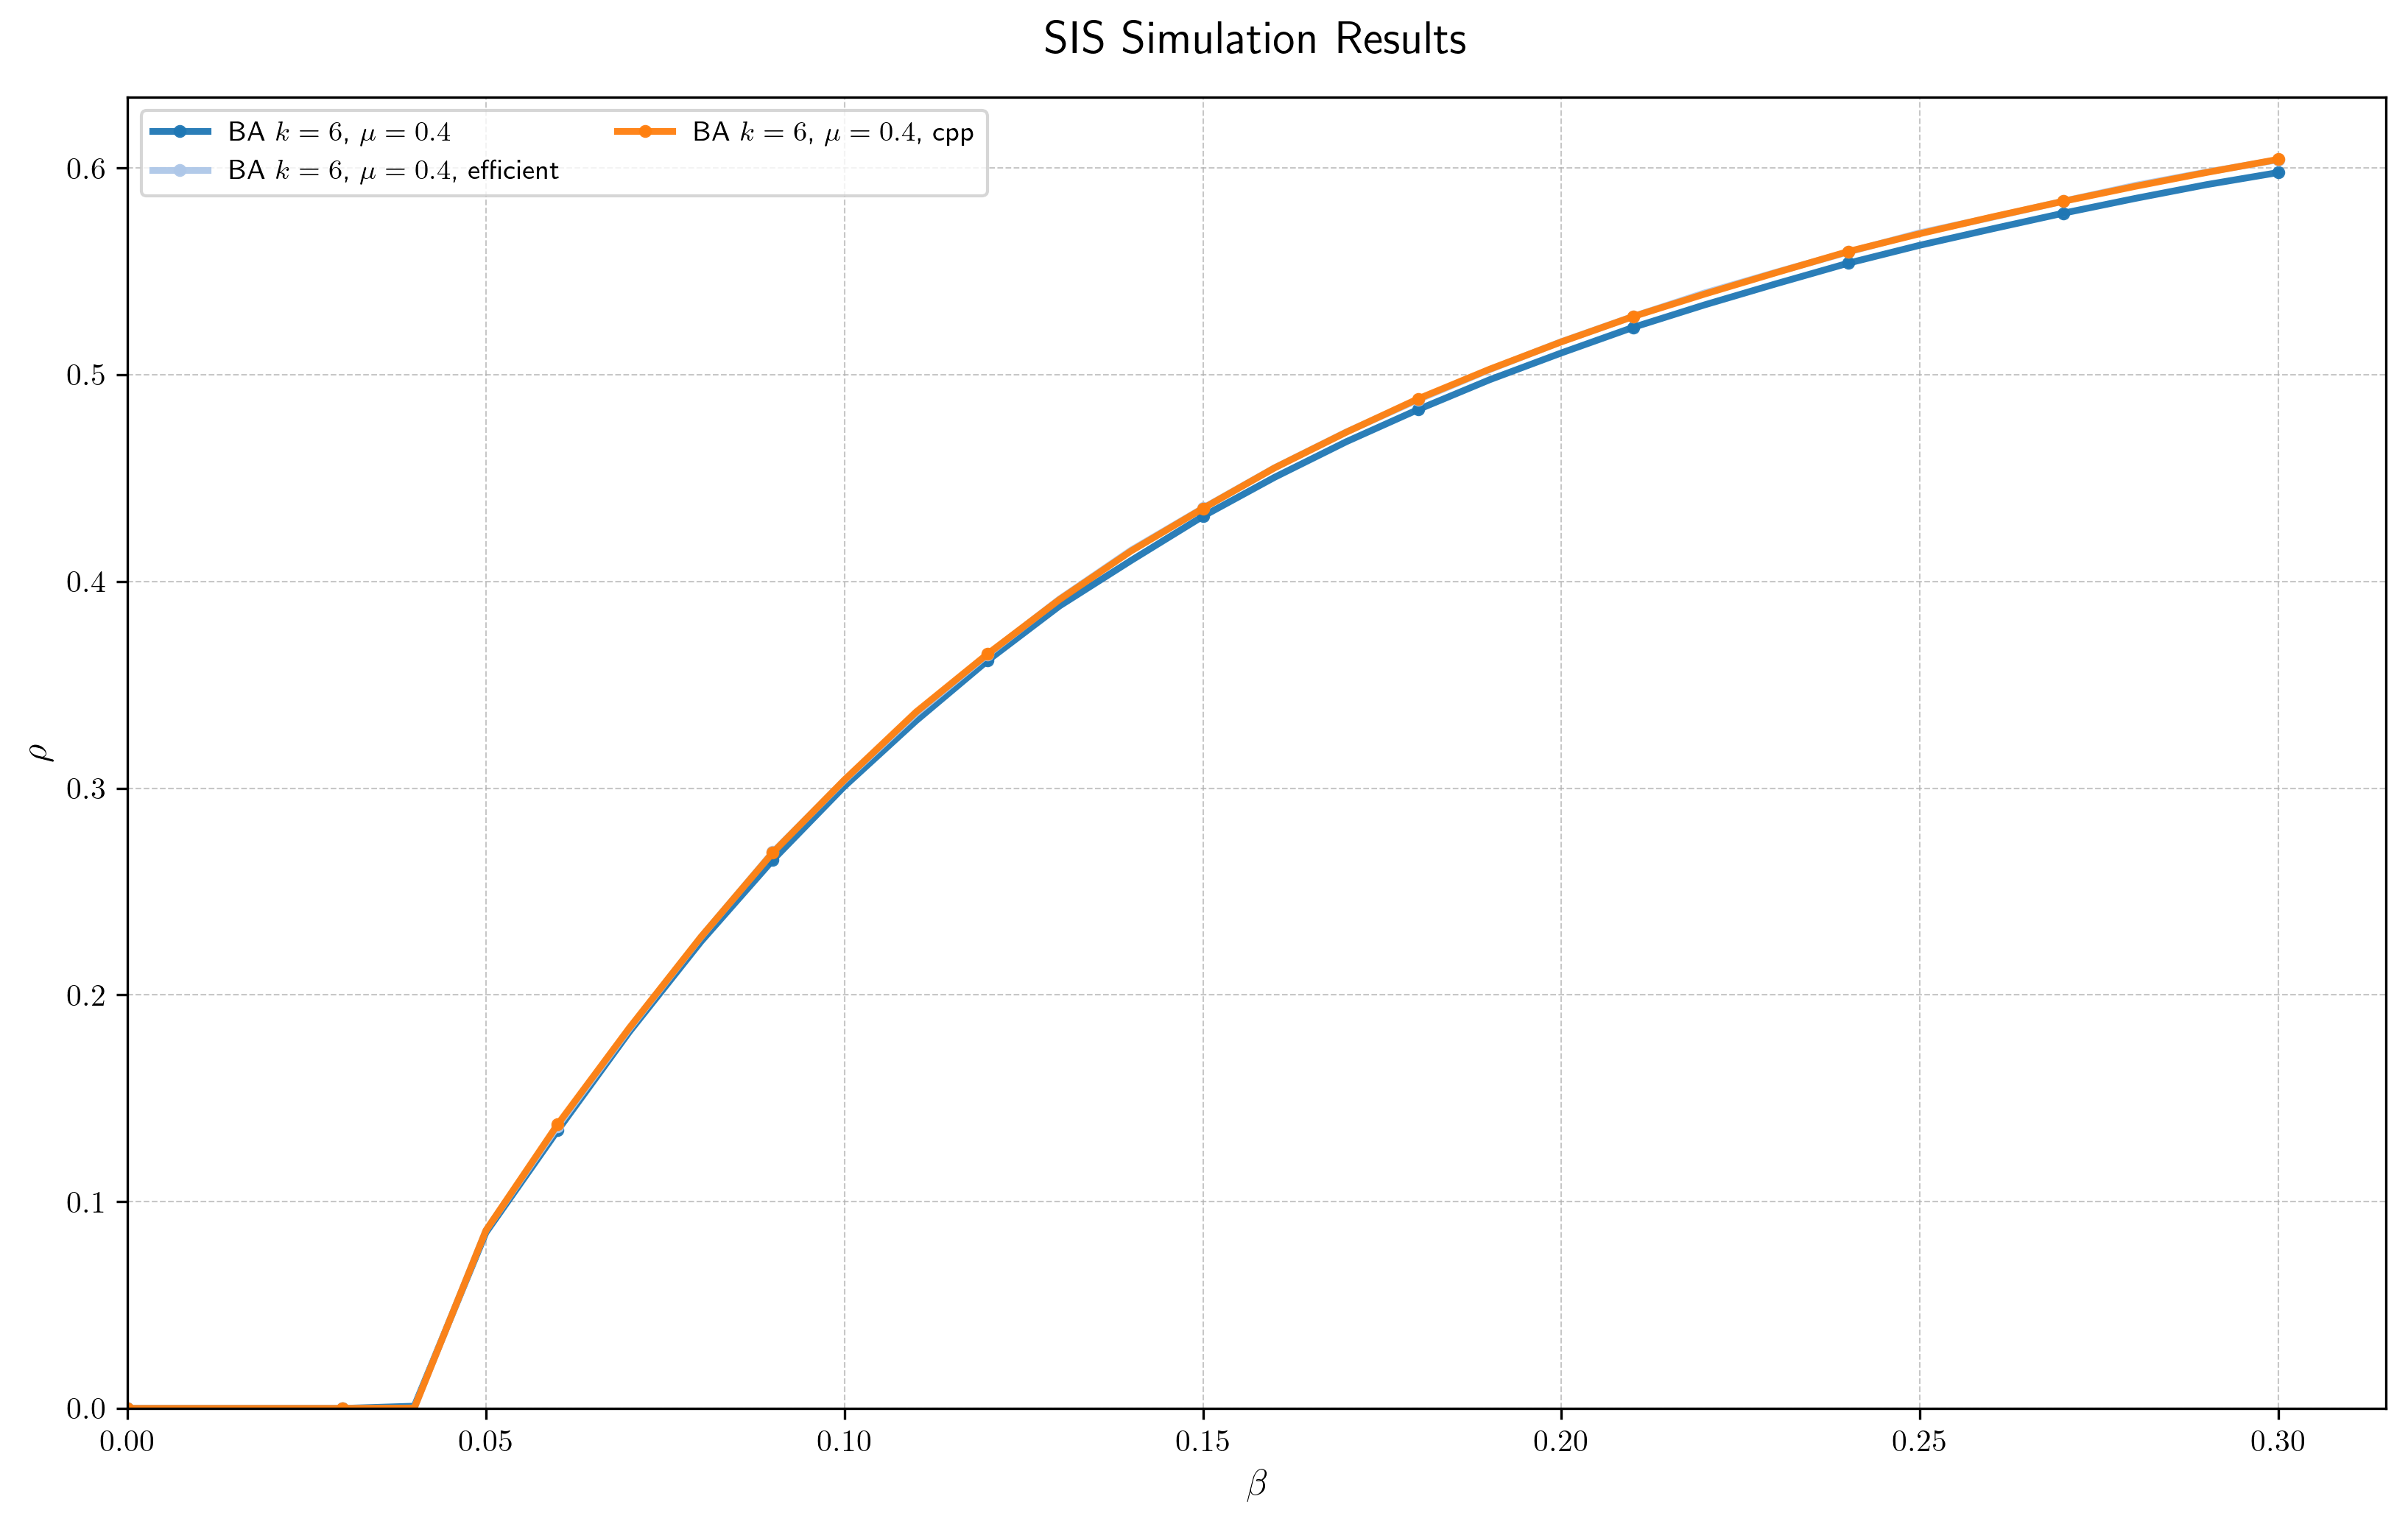
\includegraphics[width=0.85\textwidth]{assets/results_plot_graph-ba_k-6_mu-0.4_mode-all.png}
    \caption{Stationary infection density $\rho$ as a function of $\beta$ for the BA network with $\langle k \rangle = 6$ and $\mu = 0.4$, estimated by the three implementations. The curves overlap almost perfectly. Differences are due to Monte Carlo sampling variance from finite $N_{\text{rep}} = 100$.}
    \label{fig:impl_comparison}
\end{figure}

\section{Conclusion}



\newpage
\bibliography{references}


\end{document}
